\documentclass[conference]{IEEEtran}
\IEEEoverridecommandlockouts
% The preceding line is only needed to identify funding in the first footnote. If that is unneeded, please comment it out.
\usepackage{cite}
\usepackage{amsmath,amssymb,amsfonts}
\usepackage{algorithmic}
\usepackage{graphicx}
\usepackage{textcomp}
\usepackage{xcolor}

\def\BibTeX{{\rm B\kern-.05em{\sc i\kern-.025em b}\kern-.08em
    T\kern-.1667em\lower.7ex\hbox{E}\kern-.125emX}}
\begin{document}

\title{IMA205 Challenge 2023 - Report\\
{\footnotesize Student: Vitor de Sousa França}}

% \author{\IEEEauthorblockN{1\textsuperscript{st} Vitor de Sousa França}
\maketitle

\begin{abstract}
    Cardiovascular diseases are a leading cause of mortality globally, and Magnetic Resonance Imaging (MRI) is a 
    non-invasive diagnostic tool that can provide detailed information about the structure and function of the heart.
    However, manual analysis of MRI images is time-consuming and prone to bias, necessitating the development of automatic
    segmentation and classification methods to aid in diagnosis. This report describes the development and results obtained
    from the final challenge of the IMA205 subject, which involves the classification of MRI images of the heart among five
    different diagnostic classes: healthy controls, myocardial infarction, dilated cardiomyopathy, hypertrophic 
    cardiomyopathy, and abnormal right ventricle. The Automatic Cardiac Diagnosis Challenge (ACDC) dataset, which 
    comprises 150 subjects, was used for the challenge, with a training-validation set of 100 subjects and a test set of 
    50 subjects. Features were extracted from the 3D grayscale MRI images, including the perimeter of the myocardium, 
    left ventricle, right ventricle, thickness of the cardiac muscle and volumes of the myocardium, left ventricle, 
    and right ventricle. A random forest classifier was trained on these features to classify the MRI images into 
    the five diagnostic classes. The best-performing algorithm,, achieved an overall accuracy of 85.71\% in the Kaggle 
    test set. 
\end{abstract}

\begin{IEEEkeywords}
    Cardiac MRI, Feature Extraction, Machine Learning, RandomForestClassifier 
\end{IEEEkeywords}

\section{Introduction}
    Cardiovascular diseases are one of the leading causes of death globally, and their diagnosis
    and treatment are critical in improving patient outcomes. Magnetic Resonance Imaging (MRI)
    is a non-invasive diagnostic tool that can provide detailed information about the structure
    and function of the heart. Moreover, MRI is preferred over ultrasound and Computed Tomography (CT) due
    to its superior spatial-temporal resolution and non-ionizing radiation \cite{Fabian2018}.
    However, manual analysis of MRI images is time-consuming and prone to biased and non-reproducible
    outcomes. To address this, automatic segmentation and classification methods have been developed
    to aid in the diagnosis of cardiac diseases \cite{Khened2018}.

    This report presents the development and results obtained when performing the final challenge
    of the IMA205 subject. The goal of this challenge was to classify MRI images of the heart among five
    different diagnostic classes: healthy controls; myocardial infarction; dilated cardiomyopathy;
    hypertrophic cardiomyopathy; and abnormal right ventricle. The dataset provided to use in this challenge 
    was a derivation of the Automatic Cardiac Diagnosis Challenge (ACDC) dataset created from real clinical 
    exams acquired at the University Hospital of Dijon (France) \cite{Bernard2018}. It is composed of 150
    subjects, which was already randomly split into a training-validation set, with 100 subjects with
    their MRI images their corresponding segmentation and metadata (subject height and weight) and a 
    test set with 50 subjects, without the segmentation of the left-ventricle.

\section{Method}

\subsection{Feature Extraction}

    To classify the MRI images, we extracted features from them. These images are 3D and consist of 
    grayscale pixels, with the first two dimensions representing the image pixels and the third dimension 
    representing the distance, in pixels, between the slices. The images are in the NIfTI format which is 
    a well known format for storing medical imaging data. This format includes information about pixel size
    and slice distance in millimeters. The images were loaded using the nibabel library \cite{nibabel}.
    The training data included segmentation of the left and right ventricle cavity, myocardium, 
    and left ventricle, while the test data do not include the segmentation of the left ventricle cavity.
    Figures \ref{fig:diast_syst_seg_train} and \ref{fig:diast_syst_seg_test} show sample images from the
    training and test datasets, respectively.

    \begin{figure}[!ht]
    \centering
    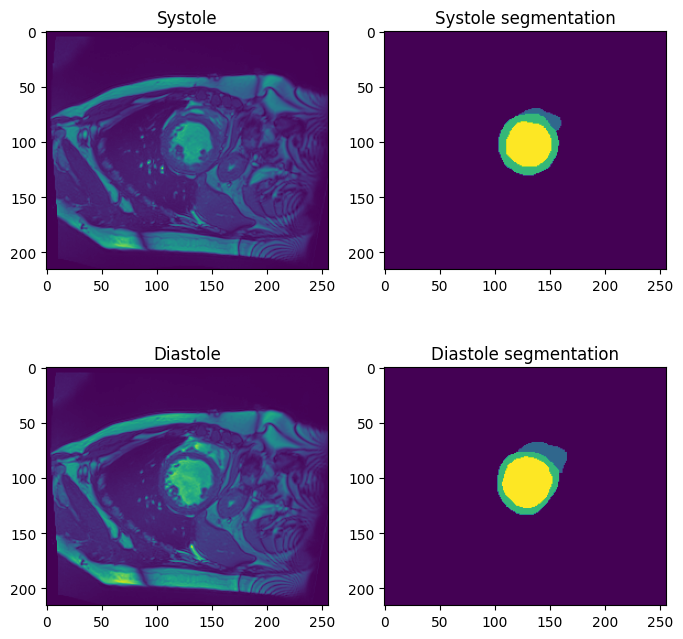
\includegraphics[width=0.5\textwidth]{images/diast_syst_seg_train.png}
    \caption{Sample MRI image from the training dataset.}
    \label{fig:diast_syst_seg_train}
    \end{figure}

    \begin{figure}[!ht]
    \centering
    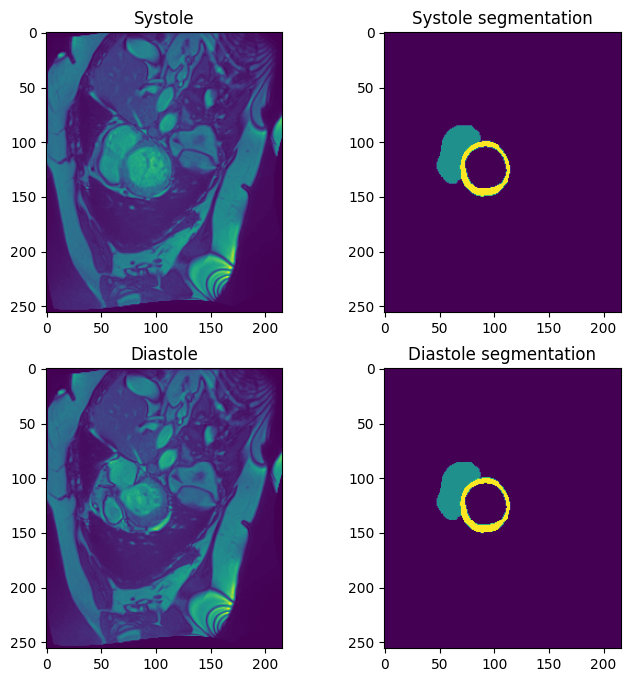
\includegraphics[width=0.5\textwidth]{images/diast_syst_seg_test.png}
    \caption{Sample MRI image from the test dataset.}
    \label{fig:diast_syst_seg_test}
    \end{figure}

    Although segmentation of the left ventricle is not mandatory for challenge criteria, 
    the features that depend on this segmentation, as the myocardium thickness, for example,
    have great relevance in classification. \cite{Khened2018, Fabian2018, Bernard2018}. So, before do the 
    feature extraction itself, it was performed the segmentation of the left ventricle in the test dataset.

    \subsubsection{Test data left ventricle segmentation}

    Since the segmentation of the myocardium was already done, the segmentation of the left ventricle
    in the test dataset was performed filling the myocardium's hole. In order to do this, it was used
    the binary fill holes function from the \textit{scipy} multidimensional image processing \cite{scipy}.
    The Figure \ref{fig:seg_test} shows a sample image from the test dataset before and after applying 
    the binary fill holes function.

    \begin{figure}[!ht]
        \centering
        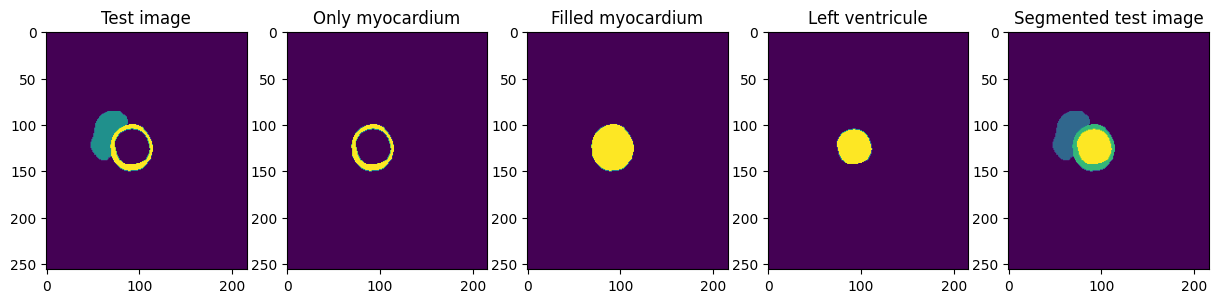
\includegraphics[width=0.5\textwidth]{images/left_vent_seg.png}
        \caption{Sample MRI image from the test dataset.}
        \label{fig:seg_test}
    \end{figure}

    After performing the segmentation on the test dataset, the same features could be extracted from the entire dataset.

    \subsubsection{Perimeter of myocardium, left ventricle and right ventricle}
        In order to obtain the perimeter of the segmentation, we employed the \textit{perimeter} method of the 
        \textit{measure} class from the \textit{scikit-image} library \cite{scikit-image}. This method returns a list of
        arrays, each representing a contour of the segmentation. The \textit{perimeter} method was applied individually 
        to each segmentation, and for each slice of the MRI image. The maximum perimeter value was obtained and recorded 
        for each subject.

    \subsubsection{Thickness of cardiac muscule}
        After obtaining the perimeters of the myocardium and left ventricle, the thickness of the cardiac muscle was
         calculated as the difference between their respective perimeters.

    \subsubsection{Volume of the myocardium, left ventricle, right ventricle}

        The volume was determined by computing the sum of the segmentation areas for each slice, which were then 
        multiplied by the pixel volume. The pixel volume was calculated by taking the inner product of the pixel size and
        the slice distance, both of which were extracted from the header of each NIfTI file.

    \subsubsection{Mass of the myocardium}

        The mass of the myocardium was calculated by multiplying the volume of the myocardium by the density of the
        myocardium. The density of the myocardium was assumed to be 1.05 g/mL \cite{Vinnakota2003}.

    \subsubsection{Left and Right Ventricle Ejection Fraction}

        As shown in the equation \ref{eq:ef}, the ejection fraction is calculated doing the division of the stroke volume
        (SV), which means the amount of blood pumped out of the ventricle at each contraction, by the end-diastolic volume
        (EDV). The stroke volume is calculated by the difference between the end-diastolic volume (EDV) and the
        end-systolic volume (ESV). 
        
        \begin{equation}
            EF = \frac{SV}{EDV} = \frac{EDV - ESV}{EDV}
            \label{eq:ef}
        \end{equation}


\subsection{Data Pre-processing}

    After the database has been prepared. A first analysis was done using the boxplot shown in
    Figure \ref{fig:data_boxplot}.

    \begin{figure}
        \centering
        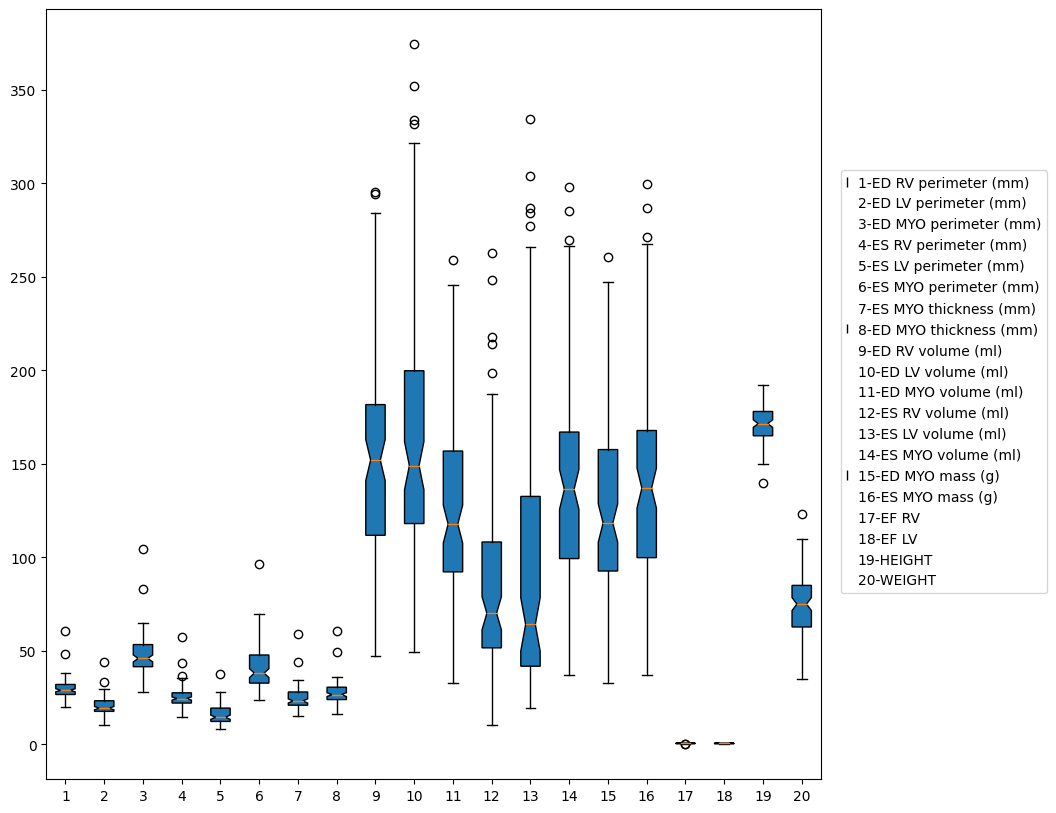
\includegraphics[width=0.5\textwidth]{images/boxplot_data.png}
        \caption{Boxplot of the training data.}
        \label{fig:data_boxplot}
    \end{figure}

    It was observed that some features have significantly different standard deviations and means.
    To avoid a bias in the model towards the features with larger orders of magnitude, it is crucial to perform 
    pre-processing on the data. Given that the data is always positive, it was chosen the normalization as pre-processing 
    step.

    The normalization was performed using the \textit{MinMaxScaler} class from the \textit{scikit-learn} library \cite{scikit-learn}.
    This class scales and translates each feature individually such that it is in the given range on the training set, 
    e.g. between zero and one. The minimum and maximum values of each feature are fitted on the training set. Then, the
    same transformation is applied to the training set and the test set. The Figure \ref{fig:data_boxplot_norm} shows the
    boxplot of the training data after the normalization.
    
    \begin{figure}
        \centering
        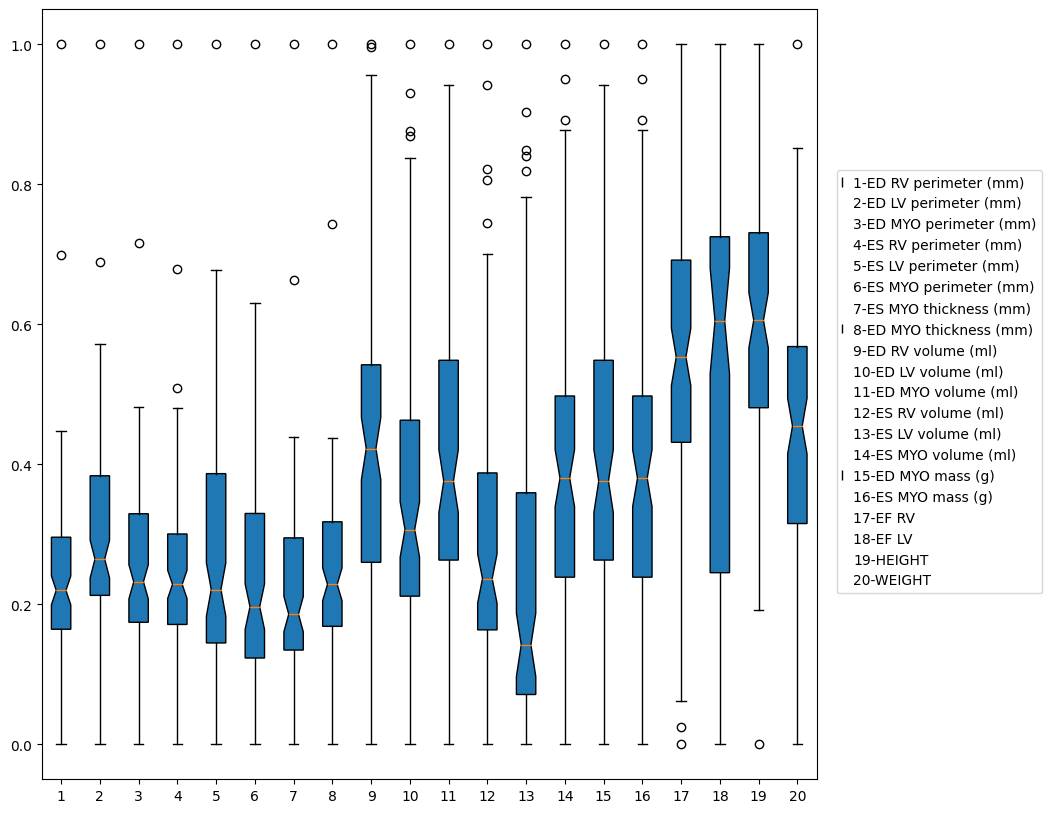
\includegraphics[width=0.5\textwidth]{images/boxplot_normalized_data.png}
        \caption{Boxplot of the training data after normalization.}
        \label{fig:data_boxplot_norm}
    \end{figure}

    
    
\subsection{Classification}
        The goal of the classification is to create an algorithm capable of classifying the patient into the possible 5 
        classes (healthy controls, myocardial infarction, dilated cardiomyopathy, hypertrophic cardiomyopathy or abnormal
        right ventricle) using the height and weight metadata and the obtained features.
       
        To achieve this, it was performed the \textit{Random Forest} algorithm. The Random Forest algorithm is 
        an ensemble learning method for classification, regression and other tasks that operates by constructing 
        a multitude of decision trees at training time and outputting the class that is the mode of the classes 
        (classification) or mean prediction (regression) of the individual trees \cite{Breiman2001}. 

        The Random Forest algorithm was selected for its robustness, low risk of overfitting, and good performance in
        classification tasks \cite{Breiman2001}. The Random Forest classifier was implemented using the 
        \textit{RandomForestClassifier} class from the \textit{scikit-learn} library \cite{scikit-learn}. This class 
        provides an implementation of the Random Forest algorithm specifically designed for classification
        tasks, and offers various parameters that can be tuned to enhance the classifier's performance.

        The parameters were first tuned using the Random Search method, which is a hyperparameter optimization technique that randomly samples candidates from a parameter 
        space with a specified distribution \cite{Bergstra2012}. The Random Search method was implemented using the 
        \textit{RandomizedSearchCV} class from the \textit{scikit-learn} library \cite{scikit-learn}. After optimizing the
        parameters with Random Search, further optimization was performed using the Grid Search method in a reduced space
        obtained by the neighborhood of the parameters previously found, which exhaustively searches through a specified
        subset of the hyperparameter space \cite{Bergstra2012}. The Grid Search method was implemented using the
        \textit{GridSearchCV} class from the \textit{scikit-learn} library \cite{scikit-learn} and was configured to perform a
        5-fold cross-validation.
        
        The parameters that were tuned are described in the next subsections.        
    
        \subsubsection{Number of estimators}
    
            The number of estimators is the number of trees in the forest. A range of 10 to 100 estimators were tested during the
            random search, with a step size of 1. The optimal number of estimators in the best performing model was found to be 15.
            Next, a grid search was conducted over 10,15,20,25,30 and 50 estimators resulting in the optimal number of estimators
            being determined as 15 again.
               
        \subsubsection{Maximum depth}
    
            The hyperparameter maximum depth of the tree refers to the maximum number of levels in a decision tree that
            the algorithm is allowed to create during the training phase. This parameter was tuned only in the Grid Search
            with a range from 2 to 8. The best performing model was found to have a maximum depth of 5. 
        
        \subsubsection{Minimum samples split}
        
            The minimum samples split is the minimum number of samples required to split an internal node.
            This parameter was tuned in the Random Search in a range of 0 to 20. The best performing model was found
            to have a minimum number of samples required to split an internal node of 5. Next, a grid search was 
            conducted in a range of 0 to 15, resulting in the optimal number of 7 samples required to split an 
            internal node.
        
        \subsubsection{Minimum samples leaf}
            
            The minimum samples leaf is the minimum number of samples required to be at a leaf node. This parameter
            was tuned in the Random Search in a range of 0 to 20. The best performing model was found to have a minimum
            number of samples required to be at a leaf node of 2. Next, a grid search was conducted in a range of
            0 to 10, resulting in the optimal number of 5 samples required to be at a leaf node.


\subsection{Results}

    The Random Forest classifier was found to be the best performing model with the following parameters: 15 estimators,
    maximum depth of 5 levels, minimum of 7 samples to split, and minimum of 5 samples to be at a leaf node.
    As the evaluation was solely based on accuracy, only this metric was taken into account. 
    The best model achieved an accuracy of 0.8571 on the Kaggle test set. 
    
    Although a confusion matrix is a useful visualization tool for algorithm performance, 
    it was not possible to plot one for the test set as it was unavailable. 
    However, the confusion matrix for the training set is presented in Figure \ref{fig:confusion_matrix}.


    \begin{figure}
        \centering
        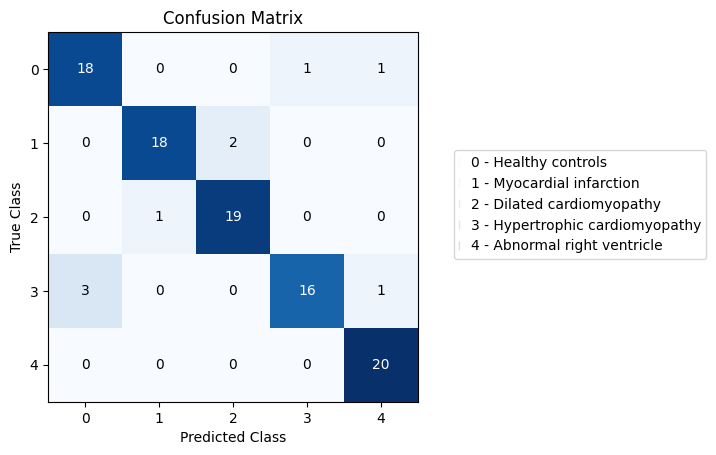
\includegraphics[width=0.5\textwidth]{images/train_cm.png}
        \caption{Confusion matrix for the train set of the best performing model.}
        \label{fig:confusion_matrix}
    \end{figure}

    Observing the confusion matrix, it is possible to see that the model has more
    difficulty in classifying the hypertrophic cardiomyopathy class comparing to the other classes.
    classifying the patient as Healthy controls in the most of the cases of error. 
    Nevertheless, just by analyzing the confusion matrix, we could say that the model classifies well for this case.
    It cannot be concluded however that it will work for unknown data, since this is the training result. 


\section{Conclusion}

    This report presented the results of the classification challenge of the IMA205 course. The goal was classifying 
    the patient into the possible 5 classes (healthy controls, myocardial infarction, dilated cardiomyopathy, hypertrophic 
    cardiomyopathy or abnormal right ventricle) using the height and weight metadata and the obtained features from a derivation 
    of the Automatic Cardiac Diagnosis Challenge (ACDC) dataset created from real clinical exams acquired at the University
    Hospital of Dijon (France). It was showed the feature extraction process, the data normalization and the classification
    where the Random Forest algorithm was used. Finally, the best model found achieved an accuracy of 85.71\% on the Kaggle 
    test set, analyzing it predictions did in the train dataset, this model had more difficulty in classifying the
    hypertrophic cardiomyopathy class comparing to the other classes, classifying the patient as Healthy controls in
    the most of the cases of error.   
   
\bibliography{IEEEabrv,mybib}
\bibliographystyle{IEEEtran}

\end{document}
